\section{Introduction}
\label{sec:intro}

\begin{figure}[t]
    \centering
    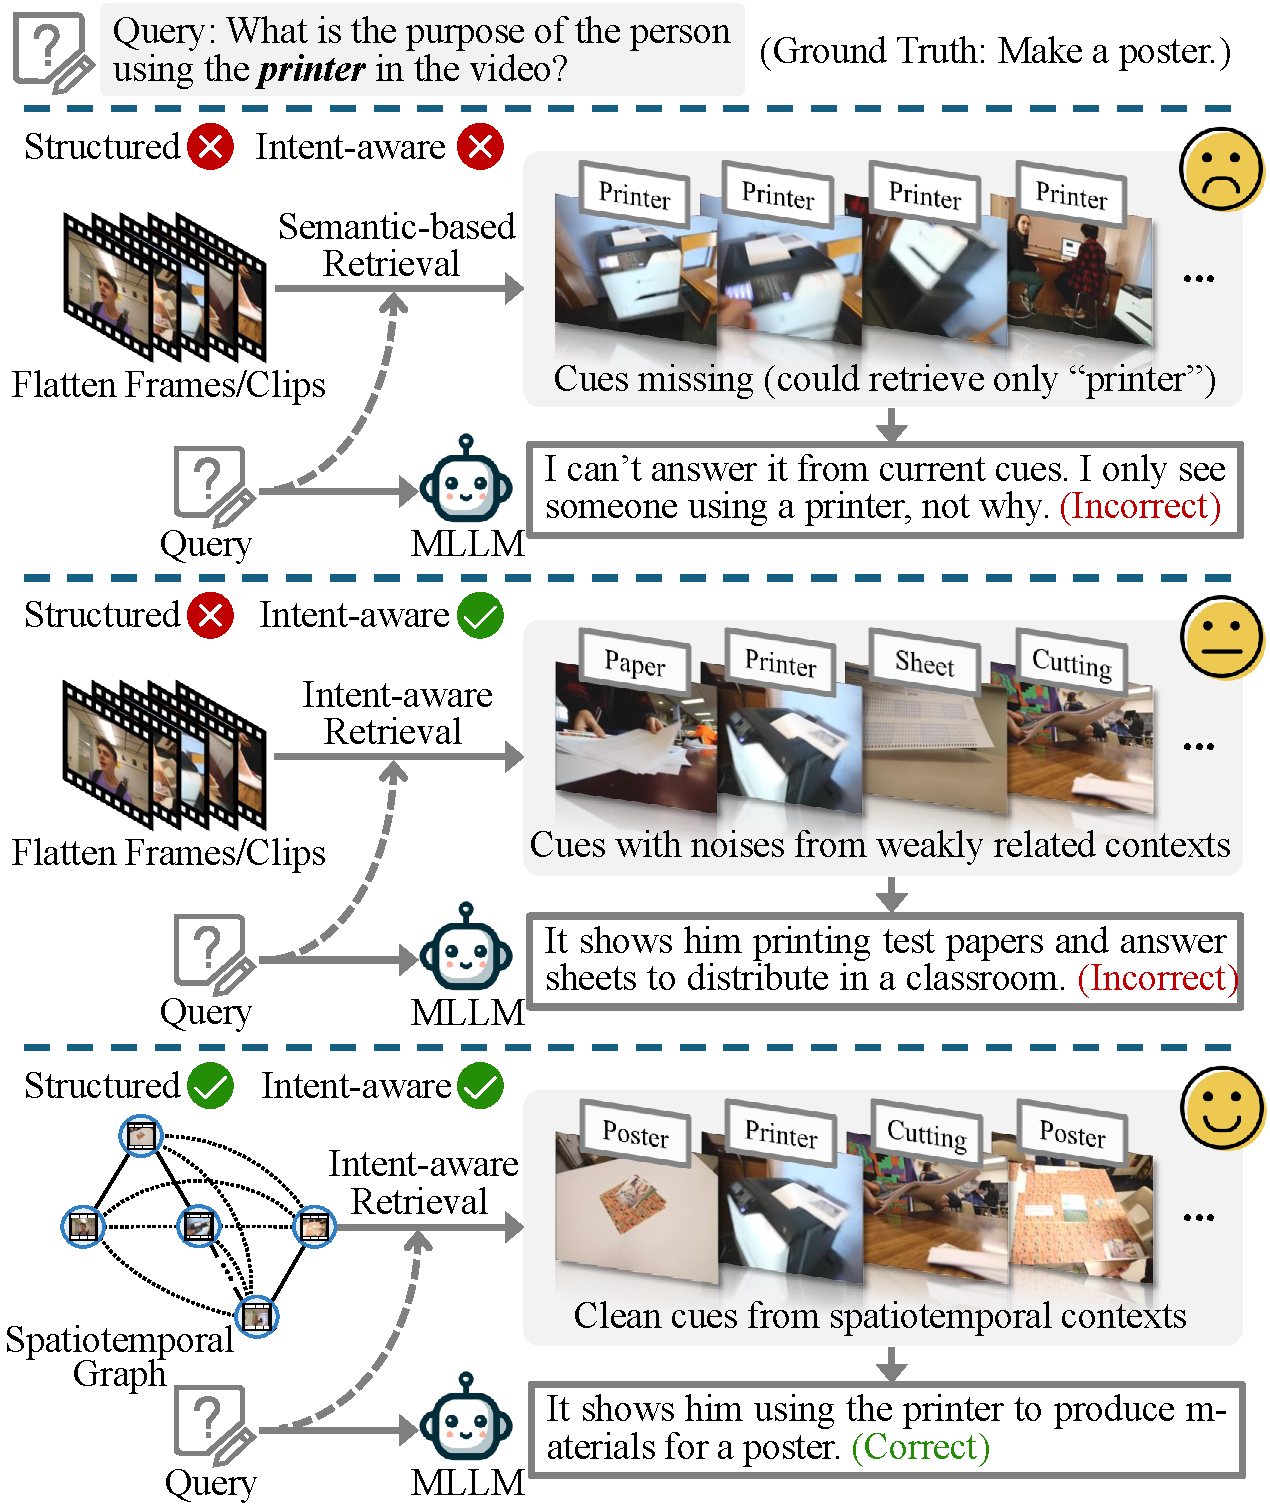
\includegraphics[width=\linewidth]{sec/figures/moti4.pdf}
    \caption{\small 
%Motivation of 
Paradigm shift from flat semantic matching to structured, intent-aware long-video RAG. \textbf{(Top)} Semantic-based retrieval relies on explicit semantic overlap, often missing cues that are only implicitly relevant to the query intent. \textbf{(Middle)} Intent-aware retrieval utilizes MLLM's reasoning capability to identify cues that may be relevant to the query intent (detailed in Sec.~\ref{sec:method_int}); however, it can be distracted by noisy cues when operating over flattened contexts scattered across long temporal ranges. \textbf{(Bottom)} VideoStir structures the video as a spatio-temporal graph to retrieve cues from coherent contexts, enabling more reliable evidence aggregation. We further discuss the benefits of structured retrieval in Fig.~\ref{fig:extended_case}.}
    \label{fig:moti}
    \vspace{-0.15in}
\end{figure}


Video understanding has emerged as a core frontier in multimodal intelligence~\cite{li2025videochat}. While recent Multimodal Large Language Models (MLLMs) have achieved {remarkable success in interpreting short clips, extending this capability to long videos remains a formidable challenge~\cite{Video-RAG}. The primary difficulty lies not merely in the video's length, but in its information density and structural complexity~\cite{vgent}. Unlike short clips that typically encapsulate a single event, long videos consist of interleaved narratives where critical cues could be sparsely scattered across the timeline. To handle the extensive contexts, state-of-the-art models often resort to expanding context windows to support uniform sampling at second level~\cite{comanici2025gemini25}.
%across long durations~\cite{comanici2025gemini25}. 
However, such approaches face a trade-off: they could either miss fine-grained details due to temporally sparse sampling or struggle with accurate reasoning when overwhelmed by redundant visual noise.}

To address the contextual intractability of processing long videos, Retrieval-Augmented Generation (RAG) has emerged as a promising solution by retrieving a small subset of segments to fit within limited context windows~\cite{exvideorag}. However, current long-video RAG methods typically flatten a video into a set of independent segments for query-based retrieval~\cite{AKS,FOCUS}, and rank candidates primarily by embedding similarity computed with contrastive vision–language models (e.g., CLIP)~\cite{clip,Video-RAG,TVRAG}. Yet this flattened semantic matching paradigm leaves two critical gaps that hinder downstream reasoning.

The first gap is \textbf{spatio-temporal structure decoupling}. Flattening a video into ndependent segments disrupts its intrinsic spatio-temporal structure, decoupling contexts that should remain linked. Because text queries may lack the fine-grained cues needed to reconnect dispersed evidence, direct matching often struggles to retrieve contexts that are spatio-temporally relevant yet share little explicit semantic overlap with the query, limiting downstream models’ ability to form coherent reasoning chains~\cite{vgent,liao2024videoinsta}. The second gap is \textbf{insufficient intent modeling}. Similarity computed from contrastive embeddings is optimized for vision–language alignment and tends to capture ``what looks similar'' rather than ``why it matters'' for addressing the query’s reasoning intent~\cite{pan2024i3}. As shown in Figure~\ref{fig:moti}, the query ``For what \textit{purpose} does the recorder use the \textit{printer}?'' leads a semantic retriever to select frames showing the ``\textit{printer}'' due to high semantic overlap, whereas the actual ``\textit{purpose}'' is revealed in a different event (e.g., making a poster), which semantic overlap alone fails to surface.


In light of these gaps, we advocate two shifts in long-video RAG paradigms: \textit{(i) From Flattened to Structured}: moving beyond isolated segment retrieval to reconstruct the intrinsic spatio-temporal topology of the video; and \textit{(ii) From Semantic to Intent}: going beyond surface semantic to model the alignment between query's intent and visual cues.

{To realize these shifts, we propose \textbf{VideoStir}, a framework designed to advance long-video RAG from flattened semantic matching to \textbf{ST}ructured, \textbf{I}ntent-aware \textbf{R}easoning.} Inspired by human episodic memory where recall proceeds coarse-to-fine (locating relevant episodes before examining details), VideoStir operates in two phases, from clips to frames. First, a coarse clip-retrieval phase addresses structure decoupling by representing the video as a spatio-temporal graph, whose nodes are semantically coherent short clips segmented by an event boundary detector. Temporal edges preserve narrative continuity, while spatial edges bridge distant yet semantically related clips via inter-clip similarity. Traversing this topology enables multi-hop retrieval from query-matched anchors to their spatio-temporal neighbors, leveraging intrinsic correlations among semantically dense clips to aggregate dependencies and mitigate the semantic sparsity of direct query matching. Second, a fine-grained frame-retrieval phase addresses insufficient intent modeling with an \textbf{I}ntent-\textbf{R}elevance scorer trained on our curated \textbf{IR-600K} dataset. Rather than considering semantic similarity alone, this lightweight MLLM-based scorer estimates frame–intent alignment, ensuring retrieved frames are not only semantically relevant but also pivotal for downstream reasoning.

Consequently, VideoStir provides the downstream MLLM with spatio-temporally context-coherent and intent-aligned visual cues, enabling more accurate long-video understanding. The scorer and curated IR-600K dataset further provide a reusable foundation for future research on intent-oriented long-video RAG systems. Our contributions are summarized as follows:

% Video understanding has emerged as a core frontier in multimodal intelligence. While recent Multimodal Large Language Models (MLLMs) have achieved remarkable success in interpreting minute-level clips, extending this capability to long videos remains a formidable challenge. The primary difficulty lies not merely in the video's length, but in its information density and structural complexity. Unlike short clips that typically encapsulate a single event, long videos consist of interleaved narratives where critical cues could be sparsely scattered across the timeline. To handle extensive contexts in long videos, state-of-the-art models often resort to expanding context windows to support uniform sampling across long durations. However, such approaches inevitably face a trade-off: they either miss fine-grained details due to sparse sampling or struggle with accurate reasoning when overwhelmed by redundant visual noise.

% To address the computational intractability of processing long-form videos, Retrieval-Augmented Generation (RAG) has emerged as a promising solution, effectively selecting relevant segments to fit within limited context windows. However, existing video RAG paradigms typically flatten the video into a collection of isolated fragments, performing retrieval based solely on semantic similarity (e.g., CLIP embeddings) with the query. This introduces two critical gaps in downstream reasoning: \textbf{(1) spatio-temporal structure decoupling.} The flattened representation of segments disrupts the intrinsic video structure, severing contexts that should remain spatio-temporally linked. As text queries often lack the fine-grained information required to re-associate such dispersed events, query-conditioned matching tends to under-retrieve spatio-temporally relevant evidence that bears weak semantic overlap to the query, limiting downstream models’ ability to form coherent reasoning chains. \textbf{(2) Insufficient intent modeling.} Current approaches mainly rely on contrastive models (e.g., CLIP) to compute embedding similarity between the query and candidate segments. Such embeddings are optimized for visual–text alignment and tend to capture ``what looks similar'' rather than ``why it matters'' for answering the query (i.e., intent-level relevance). As shown in Figure~\ref{fig:moti}, the query ``For what \textit{purpose} does the recorder use the \textit{printer}?'' leads a semantic retriever to select frames showing the \textit{printer} due to high semantic overlap, whereas the \textit{purpose} is revealed in a different event (e.g., making a poster), which semantic overlap alone fails to surface.

% In light of these gaps, we advocate two shifts in long-video RAG paradigms: \textit{(i) From Flattened to Structured}: moving beyond isolated segment retrieval to re-establish the intrinsic spatio-temporal topology of the video; and \textit{(ii) From Semantic to Intent}: going beyond surface semantic similarity to model the alignment between the query’s reasoning intent and visual content.

% To realize these shifts, we propose \textbf{VideoStir}, a framework designed to shift long-video RAG from flattened semantic matching to \textbf{ST}ructured, \textbf{I}ntent-aware \textbf{R}easoning. Inspired by human episodic memory, where recollection proceeds in a coarse-to-fine manner (locating relevant episodes before inspecting details), VideoStir operates in two phases, from clips to frames. First, a coarse clip retrieval phase addresses structure decoupling by representing the video as a spatio-temporal graph whose nodes are semantically coherent short clips obtained via a pretrained event boundary detector. Its temporal edges preserve narrative continuity, while spatial edges connect distant but semantically related clips via inter-clip self-similarity. Navigating this topology enables multi-hop retrieval from query-matched anchors to their spatio-temporal neighbors. This process leverages intrinsic correlations among semantic dense clips, aggregating dependencies through inter-clip links to mitigate the semantic sparsity of direct query-based matching. Second, a fine-grained frame retrieval phase tackles insufficient intent modeling via an intent relevance scorer trained on our curated IR-600K dataset. Instead of prioritizing semantic similarity alone, this lightweight MLLM-based scorer estimates the alignment between each frame and the query intent, ensuring that retrieved frames are not only semantically relevant but also pivotal for downstream reasoning.

% Consequently, VideoStir provides the downstream MLLM with spatio-temporally context-coherent and intent-aligned visual cues, enabling more accurate long-video understanding. Our scorer and IR-600K dataset further provide a reusable foundation for future research on intent-oriented long-video RAG systems. Our contributions are summarized as follows:


% Video understanding has emerged as a core frontier in multimodal intelligence. While recent Multimodal Large Language Models (MLLMs) have achieved strong performance on minute-level clips, extending this capability to hour-long videos raises a fundamental structural challenge. Unlike short clips that typically encapsulate a single event, long videos exhibit complex structure with extended temporal spans and dense, interleaved events. To cope with context limits, state-of-the-art MLLMs expand context windows and resort to uniform sparse sampling, which inevitably misses fine-grained cues while flooding the input with redundant frames as noise. Such noise can distract the model and impair precise reasoning. Thus, beyond simply lengthening the context, a central challenge in long-video understanding is how to efficiently select and structure visual evidence so as to bridge distant segments and disentangle interleaved events under limited contextual capacity.

% Recent research has sought to overcome these hurdles by utilizing Retrieval-Augmented Generation (RAG) for long-video understanding. By externalizing large video collections into structured textual or multimodal knowledge bases, RAG bypasses context window limits and enables scalable access to rich visual cues. However, critical gaps persist in current long-video RAG paradigms: \textbf{(1) spatio-temporal structure decoupling.} Existing methods typically flatten a long video into independent segments for query-based retrieval. This flattening disrupts the intrinsic video structure, decoupling contexts that should remain temporally and spatially linked. Because text queries could lack the fine-grained information needed to reconnect these dispersed events, direct query–video matching struggles to retrieve events that are spatio-temporally relevant but lack explicit keyword overlaps with the query. \textbf{(2) Insufficient intent modeling.} Current approaches mainly rely on contrastive models (e.g., CLIP) to compute embedding similarity between the query and candidate segments. Such embeddings are optimized for visual–text alignment and tend to capture ``what looks similar'' rather than ``why it matters'' for answering the query (i.e., intent-level relevance). As a result, retrieved candidates may exhibit high semantic similarity yet still fail to address the underlying information need, hindering downstream reasoning.

% In light of these limitations, we advocate two shifts in long-video RAG paradigms: \textit{(i) From Flattened to Structured}: moving beyond isolated segment retrieval to re-establish the intrinsic spatio-temporal topology of the video; and \textit{(ii) From Semantic to Intent}: going beyond surface semantic similarity to model the alignment between the query’s reasoning intent and visual content. Fig.~\ref{fig:moti} provides a simple illustrative example to demonstrate the motivation behind such paradigm shifts.

% To realize these shifts, we introduce \textbf{VideoStir}, a novel long-video RAG framework that retrieves pivotal visual evidence through structured \textbf{S}patiotemporal \textbf{T}opology and \textbf{I}ntent-aware \textbf{R}etrieval. Inspired by human episodic memory, where recollection proceeds in a coarse-to-fine manner (locating relevant episodes before inspecting details), VideoStir operates in two phases, from clips to frames. First, a coarse clip retrieval phase addresses structure decoupling by representing the video as a spatio-temporal graph whose nodes are semantically coherent short clips obtained via a pretrained event boundary detector. Its temporal edges preserve narrative continuity, while spatial edges connect distant but semantically related clips via inter-clip self-similarity. Navigating this topology enables multi-hop retrieval from query-matched anchors to their spatio-temporal neighbors. This process leverages intrinsic correlations among semantic dense clips, aggregating dependencies through inter-clip links to mitigate the semantic sparsity of direct query-based matching. Second, a fine-grained frame retrieval phase tackles insufficient intent modeling via an intent relevance scorer trained on our curated IR-600K dataset. Instead of prioritizing semantic similarity alone, this lightweight MLLM-based scorer estimates the alignment between each frame and the query intent, ensuring that retrieved frames are not only semantically relevant but also pivotal for downstream reasoning.

% Consequently, VideoStir provides the downstream MLLM with spatio-temporally context-coherent and intent-aligned visual cues, enabling more accurate long-video understanding. Our scorer and IR-600K dataset further provide a reusable foundation for future research on intent-oriented long-video RAG systems. Our contributions are summarized as follows:



%为什么基于相似度的检索就不能用来去捕获时空关系？例如我现在的方法是检索到一个节点之后再检索它其它的更相关的节点，那为什么我不直接相似度检索Top K?
%我的个人解释是：这是因为利用了视频内容的内部一致性Internal Consistency来补充Query的外部相关性External Relevance。即片段和片段之间的相关性，和文本和片段之间的相关性是不一样的。query检索出来的Top 3相似片段，其中Top1相似片段的自己的最相似片段可能并不是query检索出来的片段里面的东西，因为视觉模态有更多细粒度细节，因此用的Video Encoder去做这件事情。在方法部分需要讨论出来这个区别，为什么要用Video Encoder. 最好画个图表示一下，反正要说清楚这个是片段和片段间的语义计算，要说清楚片段和片段之间的内部语义计算。（例如query很简单，有主体但没有包含具体的场景，所以只能检索场景，而片段关联则可以更全面的用更加细粒度的内容去做表示，从而检索出其它相关场景。这个就用两个不同人在不同场景做例子就好，比如Top3分别对应了一个人在场景A，两个人在场景B，一个人在场景C，通过TOPk的检索可能检索出来的几个人都不在这个场景里面，但是clip关联的能够关联出这个场景的其它相关事件）
%还需要解释一下为什么要蒸馏。因为原本的效果不好。最后实验可以给一个蒸馏前后加权分数差异之类的？

\begin{itemize}
\setlength{\itemsep}{2pt}
\setlength{\parsep}{2pt}
\setlength{\parskip}{2pt}
    \item We propose VideoStir, a novel long-video RAG framework that leverages structured retrieval to reconstruct video's spatio-temporal topology and aggregate contextually coherent evidence, which overcomes the spatio-temporal decoupling of flattened retrieval.
    \item We introduce an intent-relevance scorer and IR-600K, a large-scale dataset modeling the relevance between frames and query intent. This shifts retrieval from semantic matching to intent awareness, establishing a foundation for intent-oriented long-video RAG.
    \item Extensive experiments show that VideoStir generally outperforms state-of-the-art baselines on diverse benchmarks, highlighting the promise of the paradigm shift from flattened semantic matching to structured and intent-aligned reasoning in long-video RAG.

\end{itemize}
% \begin{itemize}

%     \item We propose STC-$\text{R}^{2}$, a novel key-frame retrieval system for long videos that adaptively constructs spatio-temporal graphs to enable multi-hop semantic associations along the video timeline.
    
%     \item We develop a causal-aware Frame Reranker, which models intent-level relevance beyond semantic similarity between frames and query, significantly improving retrieval robustness and causal alignment.

%     \item We curate IR-600K, the first dataset that captures the intent-level relevance between frames and queries, offering large-scale supervision for causal-aware frame reranking and facilitating future research on long-video RAG systems.
    
% \end{itemize}

%Empirical results across diverse long-video understanding benchmarks demonstrate that STC-$\text{R}^{2}$ consistently outperforms other baselines xxxxxxx%给具体数据